\documentclass[a4paper,11pt,twoside]{scrartcl}
\usepackage[T1]{fontenc}
\usepackage{subcaption}
\usepackage[utf8]{inputenc}
\usepackage{ngerman, eucal, mathrsfs, amsfonts, bbm, amsmath, amssymb, stmaryrd,graphicx, array, geometry, color, wrapfig, wasysym, float}
\geometry{left=25mm, right=15mm, bottom=25mm}
\setlength{\parindent}{0em} 
\setlength{\headheight}{0em} 
\title{Datenbanken\\ Blatt 11}
\subtitle{Gruppe 26}
\author{Markus Vieth\and Christian Stricker}
\date{\today}
\input{../head/lstlisting.tex}
\begin{document}
\newcounter{fig}

\newcommand{\cor}[1]{\textcolor{red}{\textit{#1}}}
\newcommand{\image}[2][]{
	\begin{figure}[H]
		\centering
		\includegraphics[width=\linewidth]{#2}
		\caption{#1}
		\label{fig:Graph\thefig}
		\stepcounter{fig}
	\end{figure}
	}
\maketitle
\cleardoublepage
\pagestyle{myheadings}
\markboth{Markus Vieth, Christian Stricker}{Markus Vieth, Christian Stricker}

\section{Aufgabe}
\image[Vor dem ersten Schnitt]{./Grafik/Graph1}
\image[Nach dem ersten Schnitt]{./Grafik/Graph2}
\image[Nach dem zweiten Schnitt]{./Grafik/Graph3}
\image[Nach dem dritten Schnitt]{./Grafik/Graph4}
\image[Nach dem vierten Schnitt]{./Grafik/Graph5}
\image[Nach dem fünften Schnitt]{./Grafik/Graph6}
\image[Vor dem ersten Löschen]{./Grafik/GraphDel1}
\image[Nach dem ersten Löschen]{./Grafik/GraphDel2}
\image[Nach dem zweiten Löschen]{./Grafik/GraphDel3}
\image[Nach dem dritten Löschen]{./Grafik/GraphDel4}

\pagebreak
\section{Aufgabe}
\begin{minipage}{0.5 \textwidth}
	\subsection*{B-Baum}
\end{minipage}
\begin{minipage}{0.5 \textwidth}
	\subsection*{B+-Baum}
\end{minipage}
\subsection{Graph}
\begin{minipage}{0.5 \textwidth}
\centering
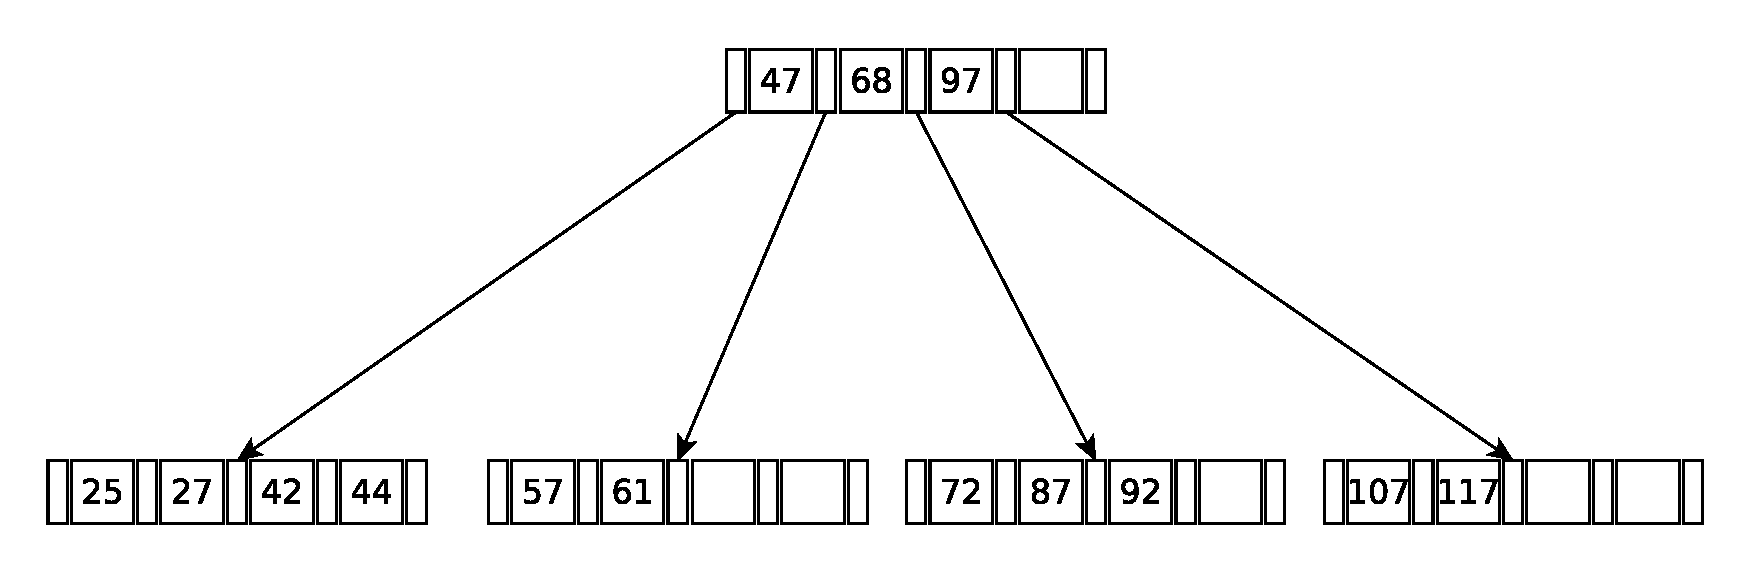
\includegraphics[width=\linewidth]{Grafik/normal.eps}
Mit k = 2
\end{minipage}
\begin{minipage}{0.5 \textwidth}
	\centering
	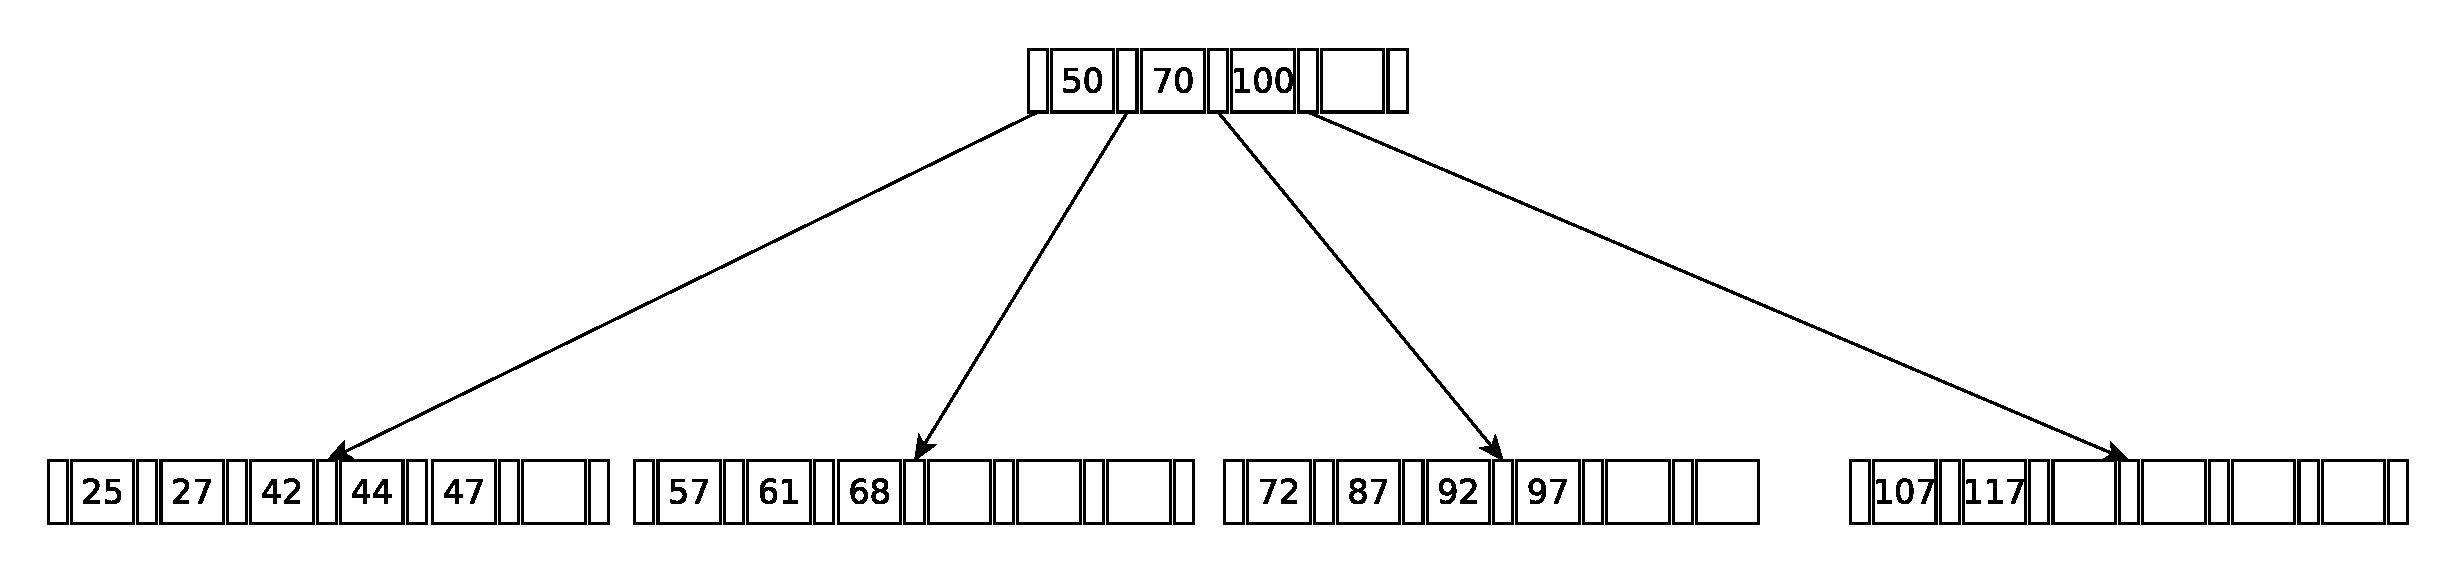
\includegraphics[width=\linewidth]{Grafik/plus.eps}
Mit k = 2 und k* = 3
\end{minipage}

\subsection{k und k*}
\begin{minipage}{0.5 \textwidth}
	k ist die minimale Anzahl an Schlüsseln in einem Knoten, welcher nicht die Wurzel ist. Ein k* existiert nicht.
\end{minipage}
\begin{minipage}{0.5 \textwidth}
	k ist die minimale Anzahl an Schlüsseln in einem Knoten, welcher nicht die Wurzel oder ein Blatt ist. k* ist die minimale Anzahl an Werten in einem Blatt.
\end{minipage}

\subsection{Innere Knoten}
\begin{minipage}{0.5 \textwidth}
	Ein innerer Knoten hat mindestens k und maximal 2k Schlüssel. Die Schlüssel sind gleichzeitig auch reale Werte. Er hat, mit n = Anzahl der Schlüssel, n+1 Kinder auf die er verweist. Die Schlüssel/Werte von Kindern, auf die "`links"' eines Schlüssel verwiesen wird, sind dabei kleiner als der betrachtete Schlüssel selbst und die rechts größer.
\end{minipage}
\begin{minipage}{0.5 \textwidth}
	Ein innerer Knoten hat mindestens k und maximal 2k Schlüssel. Ein Schlüssel entspricht dabei keinem gespeicherten Wert und müssen als solche nicht real sein. Er hat, mit n = Anzahl der Schlüssel, n+1 Kinder auf die er verweist. Die Schlüssel/Werte von Kindern, auf die "`links"' eines Schlüssel verwiesen wird, sind dabei kleiner als der betrachtete Schlüssel selbst und die rechts größer.
\end{minipage}

\subsection{Blätter}
\begin{minipage}{0.5 \textwidth}
	Ein Blatt hat mindestens k und maximal 2k Schlüssel. Die Schlüssel sind reale Werte. Es hat keine Kinder.
\end{minipage}
\begin{minipage}{0.5 \textwidth}
	Ein Blatt hat mindestens k* und maximal 2k* Schlüssel. Die Schlüssel sind reale Werte. Es hat keine Kinder.
\end{minipage}

\subsection{Höhe}
\begin{minipage}{0.5 \textwidth}
	Sei h die Höhe,n die Anzahl der Werte und k die minimale Anzahl der Schlüssel dann gilt: 
	\[ 2*(k^{h}) -1 \leq n  \leq (2k)^{h+1}-1  \]
	\[ \log_k\frac{n+1}{2}\footnote{\text{siehe Cormen S.490}} \geq h \geq \log_{2k}\;(n+1)  \]
	
	
\end{minipage}
\begin{minipage}{0.5 \textwidth}
	Sei h die Höhe,n die Anzahl der Werte und k die minimale Anzahl der Schlüssel. Die Knoten eines $B^+$ Baums haben mindestens k Schlüssel. Die Wurzel hat mindestens 1 Schlüssel und somit 2 Kinder. Ein Knoten hat mehr als k Kinder, somit gilt : 
	\[ n \geq 2 k^{h + 1}   \]
	\[ \log_k \frac{n}{2} \geq h  \]
\end{minipage}
\pagebreak
\section{Aufgabe}
Daten in Datenbanken sind meist nicht nur durch ein Attribut definiert, sondern durch mehrere.
Um nun zu ermöglichen, Daten durch Abfragen in Bereichen in mehreren Attributen effizient zu beziehen, werden R-Bäume verwendet.
In einem R-Baum werden Daten durch mehrdimensionale Objekte(2D Polygone, 3D geometrische Körper) gespeichert.
Jedes Level eines R-Baumes grenzt dabei den betrachteten Bereich weiter ein, bis die Daten eindeutig bestimmt werden können.
Dadurch ist es möglich effizient Bereichsanfragen zu bearbeiten.
Wie auch die B-Bäume, sind die R-Bäume balanciert und als solche effizient in der Suche.
Auch die interne Struktur ähnelt den B-Bäumen und ist genau wie diese dynamisch, passt sich also Änderungen in der Datenmenge an.
Über die räumliche Abstraktion ist es möglich über die geometrische Distanz effizient den nächsten Nachbarn eines Wertes zu bestimmen.
\end{document}